\hypertarget{bausteinsicht}{%
\section{Bausteinsicht}\label{bausteinsicht}}

\textbf{Inhalt}

Diese Sicht zeigt die statische Zerlegung des Systems in Bausteine sowie
deren Beziehungen. Beispiele für Bausteine sind unter anderem:

\begin{itemize}
\tightlist
\item
  Module
\item
  Komponenten
\item
  Subsysteme
\item
  Klassen
\item
  Interfaces
\item
  Pakete
\item
  Bibliotheken
\item
  Frameworks
\item
  Schichten
\item
  Partitionen
\item
  Tiers
\item
  Funktionen
\item
  Makros
\item
  Operationen
\item
  Datenstrukturen
\item
  \ldots{}
\end{itemize}

Diese Sicht sollte in jeder Architekturdokumentation vorhanden sein. In
der Analogie zum Hausbau bildet die Bausteinsicht den
\emph{Grundrissplan}.

\textbf{Motivation}

Behalten Sie den Überblick über den Quellcode, indem Sie die statische
Struktur des Systems durch Abstraktion verständlich machen.

Damit ermöglichen Sie Kommunikation auf abstrakterer Ebene, ohne zu
viele Implementierungsdetails offenlegen zu müssen.

\textbf{Form}

Die Bausteinsicht ist eine hierarchische Sammlung von Blackboxen und
Whiteboxen (siehe Abbildung unten) und deren Beschreibungen.

\begin{figure}
\centering
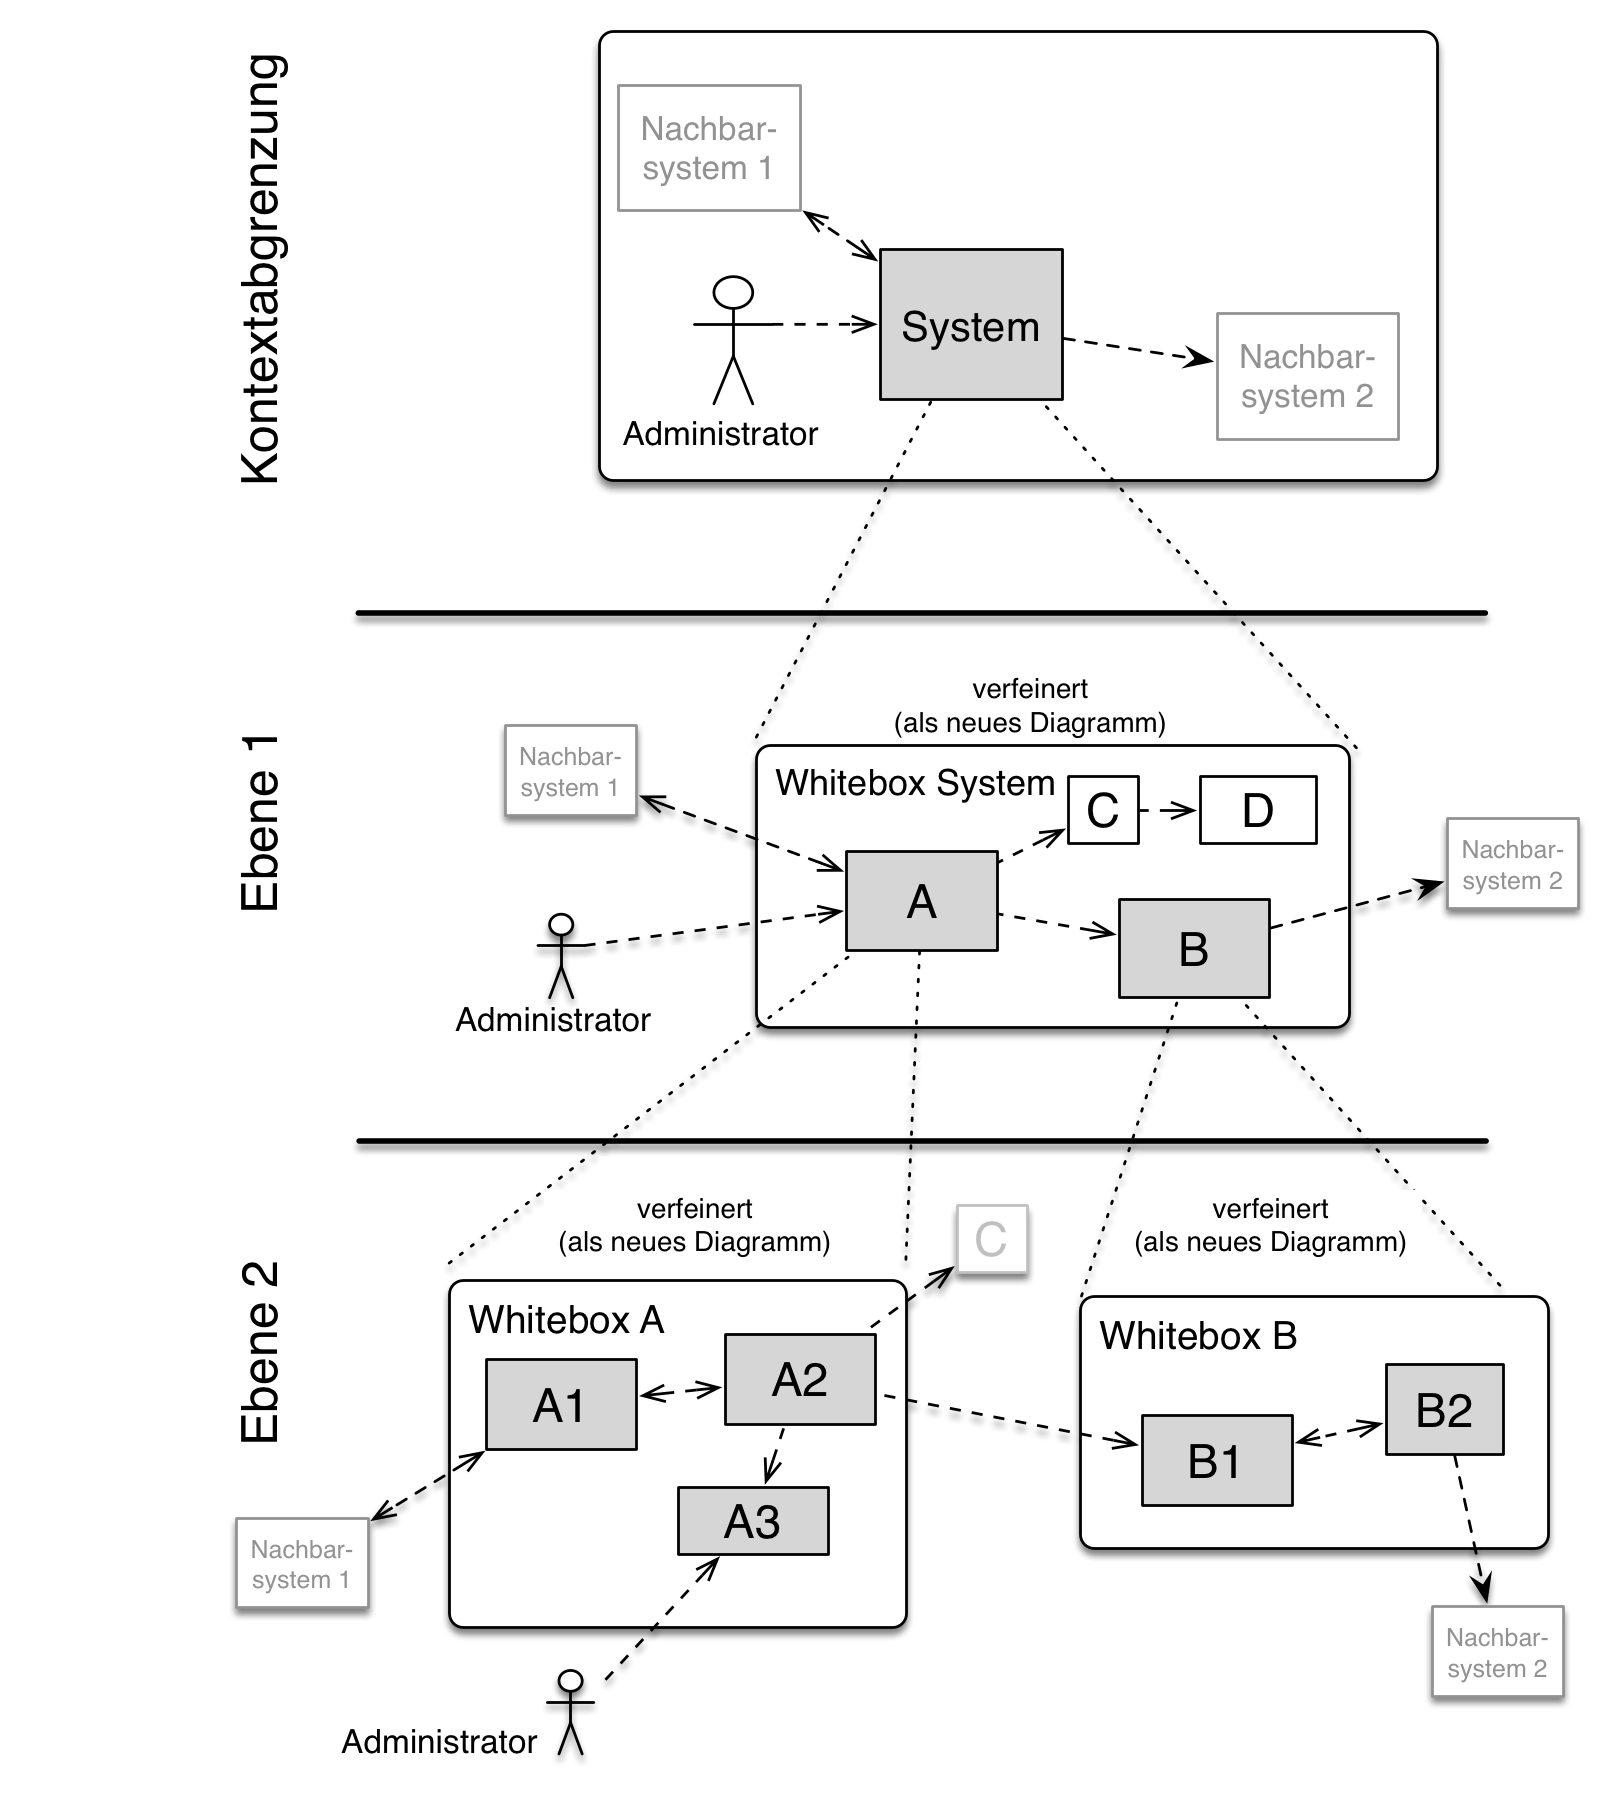
\includegraphics{../images/05_building_blocks-DE.png}
\caption{Baustein Sichten}
\end{figure}

\textbf{Ebene 1} ist die Whitebox-Beschreibung des Gesamtsystems,
zusammen mit Blackbox-Beschreibungen der darin enthaltenen Bausteine.

\textbf{Ebene 2} zoomt in einige Bausteine der Ebene 1 hinein. Sie
enthält somit die Whitebox-Beschreibungen ausgewählter Bausteine der
Ebene 1, jeweils zusammen mit Blackbox-Beschreibungen darin enthaltener
Bausteine.

\textbf{Ebene 3} zoomt in einige Bausteine der Ebene 2 hinein, usw.

\hypertarget{whitebox-gesamtsystem}{%
\subsection{Whitebox Gesamtsystem}\label{whitebox-gesamtsystem}}

An dieser Stelle beschreiben Sie die Zerlegung des Gesamtsystems anhand
des nachfolgenden Whitebox-Templates. Dieses enthält:

\begin{itemize}
\tightlist
\item
  Ein Übersichtsdiagramm
\item
  die Begründung dieser Zerlegung
\item
  Blackbox-Beschreibungen der hier enthaltenen Bausteine. Dafür haben
  Sie verschiedene Optionen:

  \begin{itemize}
  \tightlist
  \item
    in \emph{einer} Tabelle, gibt einen kurzen und pragmatischen
    Überblick über die enthaltenen Bausteine sowie deren Schnittstellen.
  \item
    als Liste von Blackbox-Beschreibungen der Bausteine, gemäß dem
    Blackbox-Template (siehe unten). Diese Liste können Sie, je nach
    Werkzeug, etwa in Form von Unterkapiteln (Text), Unter-Seiten (Wiki)
    oder geschachtelten Elementen (Modellierungswerkzeug) darstellen.
  \end{itemize}
\item
  (optional:) wichtige Schnittstellen, die nicht bereits im
  Blackbox-Template eines der Bausteine erläutert werden, aber für das
  Verständnis der Whitebox von zentraler Bedeutung sind. Aufgrund der
  vielfältigen Möglichkeiten oder Ausprägungen von Schnittstellen geben
  wir hierzu kein weiteres Template vor. Im schlimmsten Fall müssen Sie
  Syntax, Semantik, Protokolle, Fehlerverhalten, Restriktionen,
  Versionen, Qualitätseigenschaften, notwendige Kompatibilitäten und
  vieles mehr spezifizieren oder beschreiben. Im besten Fall kommen Sie
  mit Beispielen oder einfachen Signaturen zurecht.
\end{itemize}

\textbf{\emph{\textless Übersichtsdiagramm\textgreater{}}}

\begin{description}
\item[Begründung]
\emph{\textless Erläuternder Text\textgreater{}}
\item[Enthaltene Bausteine]
\emph{\textless Beschreibung der enthaltenen Bausteine
(Blackboxen)\textgreater{}}
\item[Wichtige Schnittstellen]
\emph{\textless Beschreibung wichtiger Schnittstellen\textgreater{}}
\end{description}

Hier folgen jetzt Erläuterungen zu Blackboxen der Ebene 1.

Falls Sie die tabellarische Beschreibung wählen, so werden Blackboxen
darin nur mit Name und Verantwortung nach folgendem Muster beschrieben:

\begin{longtable}[]{@{}ll@{}}
\toprule
Name & Verantwortung\tabularnewline
\midrule
\endhead
\emph{\textless Blackbox 1\textgreater{}} &
\emph{\textless Text\textgreater{}}\tabularnewline
\emph{\textless Blackbox 2\textgreater{}} &
\emph{\textless Text\textgreater{}}\tabularnewline
\bottomrule
\end{longtable}

Falls Sie die ausführliche Liste von Blackbox-Beschreibungen wählen,
beschreiben Sie jede wichtige Blackbox in einem eigenen
Blackbox-Template. Dessen Überschrift ist jeweils der Namen dieser
Blackbox.

\textbf{\textless Name Blackbox 1\textgreater{}}

Beschreiben Sie die \textless Blackbox 1\textgreater{} anhand des
folgenden Blackbox-Templates:

\begin{itemize}
\tightlist
\item
  Zweck/Verantwortung
\item
  Schnittstelle(n), sofern diese nicht als eigenständige Beschreibungen
  herausgezogen sind. Hierzu gehören eventuell auch Qualitäts- und
  Leistungsmerkmale dieser Schnittstelle.
\item
  (Optional) Qualitäts-/Leistungsmerkmale der Blackbox, beispielsweise
  Verfügbarkeit, Laufzeitverhalten o. Ä.
\item
  (Optional) Ablageort/Datei(en)
\item
  (Optional) Erfüllte Anforderungen, falls Sie Traceability zu
  Anforderungen benötigen.
\item
  (Optional) Offene Punkte/Probleme/Risiken
\end{itemize}

\emph{\textless Zweck/Verantwortung\textgreater{}}

\emph{\textless Schnittstelle(n)\textgreater{}}

\emph{\textless(Optional) Qualitäts-/Leistungsmerkmale\textgreater{}}

\emph{\textless(Optional) Ablageort/Datei(en)\textgreater{}}

\emph{\textless(Optional) Erfüllte Anforderungen\textgreater{}}

\emph{\textless(optional) Offene Punkte/Probleme/Risiken\textgreater{}}

\textbf{\textless Name Blackbox 2\textgreater{}}

\emph{\textless Blackbox-Template\textgreater{}}

\textbf{\textless Name Blackbox n\textgreater{}}

\emph{\textless Blackbox-Template\textgreater{}}

\textbf{\textless Name Schnittstelle 1\textgreater{}}

\ldots{}

\textbf{\textless Name Schnittstelle m\textgreater{}}

\hypertarget{ebene-2}{%
\subsection{Ebene 2}\label{ebene-2}}

Beschreiben Sie den inneren Aufbau (einiger) Bausteine aus Ebene 1 als
Whitebox.

Welche Bausteine Ihres Systems Sie hier beschreiben, müssen Sie selbst
entscheiden. Bitte stellen Sie dabei Relevanz vor Vollständigkeit.
Skizzieren Sie wichtige, überraschende, riskante, komplexe oder
besonders volatile Bausteine. Normale, einfache oder standardisierte
Teile sollten Sie weglassen.

\textbf{Whitebox \emph{\textless Baustein 1\textgreater{}}}

\ldots zeigt das Innenleben von \emph{Baustein 1}.

\emph{\textless Whitebox-Template\textgreater{}}

\textbf{Whitebox \emph{\textless Baustein 2\textgreater{}}}

\emph{\textless Whitebox-Template\textgreater{}}

\ldots{}

\textbf{Whitebox \emph{\textless Baustein m\textgreater{}}}

\emph{\textless Whitebox-Template\textgreater{}}

\hypertarget{ebene-3}{%
\subsection{Ebene 3}\label{ebene-3}}

Beschreiben Sie den inneren Aufbau (einiger) Bausteine aus Ebene 2 als
Whitebox.

Bei tieferen Gliederungen der Architektur kopieren Sie diesen Teil von
arc42 für die weiteren Ebenen.

\textbf{Whitebox \textless\_Baustein x.1\_\textgreater{}}

\ldots zeigt das Innenleben von \emph{Baustein x.1}.

\emph{\textless Whitebox-Template\textgreater{}}

\textbf{Whitebox \textless\_Baustein x.2\_\textgreater{}}

\emph{\textless Whitebox-Template\textgreater{}}

\textbf{Whitebox \textless\_Baustein y.1\_\textgreater{}}

\emph{\textless Whitebox-Template\textgreater{}}
